\section{Моделирование и оптимизация двухкубитных логических операций}
\label{sec:chapter_4}

Двухкубитные операции квантового компьютера на нейтральных атомах реализуются с помощью механизма ридберговской блокады, при которой два близко находящихся атома не могут быть возбуждены в ридберговское состояние одновременно. В работе моделируется двухфотонное возбуждение одиночных атомов в ридберговское состояние с учётом различных механизмов декогеренции: динамика атома в оптическом пинцете, эффект Доплера, спонтанный распад из промежуточного состояния [1], фазовые шумы лазера [2]. Результаты моделирования позволяют подобрать оптимальные параметры двухфотонного возбуждения и определить основные факторы, ограничивающие точность двухкубитных операций нашей установки.

\subsection{Ридберговская блокада, нативный гейт CZ}

Для того чтобы понять принцип реализации двухкубитных гейтов с помощью ридберговской блокады рассмотрим гамильтониан двух атомов с кубитными уровнями $\ket{0}, \; \ket{1}$ и дополнительным ридберговским уровнем $\ket{r}$. Будем одновременно светить на оба атома лазером резонансным с переходом $\ket{1} \leftrightarrow \ket{r}$. Гамильтониан такой системы в приближении вращающейся волны без учёта взаимодействия между атомами запишется как 

\begin{equation}
	\hat{H}_0 = \sum_{i=1,2}\frac{\Omega}{2}\left(e^{i\phi}\ket{1_i}\bra{r_i} + e^{-i\phi}\ket{r_i}\bra{i_i}\right)-\Delta \ket{r_i}\bra{r_i},
\end{equation}

где $\Omega e^{i\phi}$ - частота Раби, $\Delta$ - отстройка от резонанса $\ket{1} \leftrightarrow \ket{r}$. Если нейтральные атомы находятся в кубитных состояниях $\ket{0},\; \ket{1}$, либо в ридберговском состоянии $\ket{r}$ находится лишь один из атомов, то диполь-дипольным взаимодействием между ними можно пренебречь, так как расстояние между атомами составляет $r_0 = 3.4 \text{ мкм}$, что сильно меньше характерного размера атома (порядка нескольких ангстремов). Если же оба атома одновременно находятся в высоковозбужденном ридберговском состоянии $\ket{r}$ с главным квантовым числом порядка $50-100$, то диполь-дипольное взаимодействие сильно вырастает. Скорость роста диполь-дипольного взаимодействия от расстояния между атомами $\vec{r}_0$ можно оценить следующим образом. Энергия взаимодействия двух классических точечных диполей равна

\begin{equation}
	V_{dip} = \frac{\vec{d}_1 \cdot \vec{d}_2}{r_0^3} - 3\frac{\left(\vec{d}_1, \vec{r}_0\right)\left(\vec{d}_2, \vec{r}_0\right)}{r_0^5}.
\end{equation}

Атом $^{87}\text{Rb}$ является водородоподобным, так как имеет один валентный электрон, то есть характерный размер атома (электронного облака) зависит от главного квантового числа как $n^2$ (боровские орбиты). Отсюда следует, что величина дипольного момента атома также растёт как $n^2$, то есть для величины диполь-дипольного взаимодействия получаем 

\begin{equation}
	V_{dip} \sim \frac{n^4}{r_0^3}. 
\end{equation}

В квантовом случае дипольные моменты атомов нужно заменить на соответствующие операторы дипольного момента. Для водородоподобных атомов среднее значение дипольного момента зануляется в силу определённой четности волновых функций \cite{Belousov} относительно инверсии координаты $\vec{r} \rightarrow -\vec{r}$. Пусть $\psi(\vec{r})$ - координатное представление некоторой собственной волновой функции с определённой четностью (чётная или нечётная относительно инверсии координаты), тогда среднее значение дипольного момента запишется как

\begin{equation}
	\left< \hat{\vec{d}}\;\right> = \bra{\psi}\left( e \hat{\vec{r}}\right)\ket{\psi} = e\int_{\mathbb{R}^3}|\psi(\vec{r})|^2\vec{r} \; d^3\vec{r}.
\end{equation}

Видно, что под интегралом по всему пространству стоит произведение чётной функции $|\psi(\vec{r})|^2$ относительно инверсии координаты на нечётную $\vec{r}$, то есть среднее значение дипольного момента зануляется. Отсюда следует, что диполь-дипольное взаимодействие между нейтральными атомами в невырожденной теории возмущений проявляется только во втором порядке, то есть 

\begin{equation}
	V \sim V_{dip}^2 \sim \frac{n^8}{r_0^6}.
\end{equation}

Так как диполь-дипольное взаимодействие проявляется только в случае когда оба атома находятся в ридберговском состоянии, то можно ввести оператор взаимодействия между двумя атомами как 

\begin{equation}
	\hat{V} = V \ket{r_1}\bra{r_1}\otimes \ket{r_2}\bra{r_2}.
\end{equation}

Отсюда получается полный ридберговский гамильтониан как 

\begin{equation}
	\hat{H} = \hat{H}_0 + \hat{V} = \sum_{i=1,2}\left\{ \frac{\Omega}{2}\left(e^{i\phi}\ket{1_i}\bra{r_i} + e^{-i\phi}\ket{r_i}\bra{1_i}\right)-\Delta \ket{r_i}\bra{r_i}\right\} + V \ket{r_1}\bra{r_1}\otimes \ket{r_2}\bra{r_2}.
\end{equation}

Видно, что гамильтониан никак не действует на атом в состоянии $\ket{0}$, то есть двухчастичное состояние $\ket{00}$ не эволюционирует. Для пар состояний $\ket{01}, \; \ket{0r}$ и $\ket{10}, \; \ket{r0}$ ридберговский гамильтониан сводится к одночастичному 

\begin{equation}
	\hat{H}_{1} = \frac{\Omega}{2}\left(e^{i\phi}\ket{1}\bra{r} + e^{-i\phi}\ket{r}\bra{1}\right)-\Delta \ket{r}\bra{r}, 
\end{equation}

то есть наблюдаются обычные осцилляции Раби для переходов $\ket{01} \leftrightarrow \ket{0r}$ и $\ket{10}\leftrightarrow \ket{r0}$. Ситуация с состояниями $\ket{11}, \; \ket{1r}, \; \ket{r1}, \;\ket{rr}$ более интересна. Рассмотрим предел сильного ридберговского взаимодействия между атомами $V \gg \Omega, \Delta$. Такой режим как раз реализуется в нашей установке при расстоянии между атомами $r_0 = 3.4 \text{ мкм}$. Посмотрим как гамильтониан действует на эти состояния по отдельности 


\begin{equation}
	\begin{aligned}
		\hat{H} & \ket{11} = \frac{\Omega}{2}e^{-i\phi}\left(\ket{r1} + \ket{1r}\right) = \frac{\sqrt{2}\Omega}{2}e^{-i\phi}\ket{w},\\
		\hat{H} & \ket{1r} = -\Delta \ket{1r} + \frac{\Omega}{2}e^{-i\phi}\ket{rr} + \frac{\Omega}{2}e^{i\phi}\ket{11}, \\
		\hat{H} & \ket{w} = -\sqrt{2}\Delta \ket{w} + \frac{\sqrt{2}\Omega}{2}e^{-i\phi}\ket{rr} + \frac{\sqrt{2}\Omega}{2}e^{i\phi}\ket{11}   ,\\
		\hat{H} & \ket{rr} = (V-2\Delta)\ket{rr} + \frac{\sqrt{2}\Omega}{2}e^{i\phi}\ket{w}, \\
		& \ket{w} = \frac{1}{\sqrt{2}}\left(\ket{r1} + \ket{1r}\right).
	\end{aligned}
\end{equation}

Таким образом, гамильтониан распадается на две части

\begin{equation}
	\begin{aligned}
		& \hat{H}_{2} = -\sqrt{2}\Delta \ket{w}\bra{w} + \frac{\sqrt{2}\Omega}{2}\left(e^{i\phi}\ket{11}\bra{w} +e^{-i\phi}\ket{w}\bra{11} \right), \\
		& \hat{H}_{3} = (V-2\Delta)\ket{rr}\bra{rr} + \frac{\sqrt{2}\Omega}{2}\left(e^{i\phi}\ket{w}\bra{rr} +e^{-i\phi}\ket{rr}\bra{w} \right).
	\end{aligned}
\end{equation}

Видно что получились стандартные гамильтонианы Раби для переходов $\ket{11} \leftrightarrow \ket{w}$ и $\ket{w} \leftrightarrow \ket{rr}$. При условии $V \gg \Delta, \Omega$ гамильтониан $\hat{H}_3$ соответствует случаю сильной отстройки от резонанса, то есть осцилляции Раби между состояниями $\ket{w}$ и $\ket{rr}$ не происходят. Отсюда получается, что можно оставить только гамильтониан $H_2$, то есть будут происходить осцилляции Раби между двухуровневой системой $\ket{11}, \; \ket{w}$. Физически это соответсвует тому, что одновременное возбуждение в ридберговское состояние требует дополнительной энергии $V$, то есть такой переход не идёт. Вместо этого в ридберговское состояние возбуждается лишь один атом, что в квантовом случае соответствует равновероятной суперпозиции $\ket{1r}$ и $\ket{r1}$. Этот эффект называется эффектом ридберговской блокады. Также можно отметить, что состояние $\ket{w}$ это максимально запутанное состояние Бэлла двух атомов в базисе $\ket{1}, \; \ket{r}$, то есть за счёт эффекта ридберговской блокады удаётся контроллируемым образом передать запутанность между двумя атомами. Осталось теперь перевести атомы в кубитный базис, сохранив заупатнность. Это можно сделать с помощью последовательности Levine-Pichler \cite{toffoli}, которая реализует нативный $CZ$-гейт. На рисунке \ref{fig:LP_total} показана схема последовательности Levine-Pichler, для её реализации требуется выставить следующие параметры \cite{toffoli}

\begin{equation}
	\begin{aligned}
		& \Delta/\Omega = 0.377371, \\
		& \xi = 3.90242, \\
		& \Omega \tau = 4.29268.
	\end{aligned}
\end{equation}

Последовательность состоит из двух одинаковых импульсов с изменением фазы частоты Раби $\Omega \rightarrow \Omega e^{i\xi}$ между ними, в итоге получается гейт $CZ$ в базисе $\ket{00}, \; \ket{01}, \; \ket{10}, \; \ket{11}$ 

\begin{equation}
	CZ = \begin{pmatrix}
		1 & 0 & 0 & 0\\
		0 & 1 & 0 & 0\\
		0 & 0 & 0 & 1\\
		0 & 0 & 0 & -1
	\end{pmatrix}.
\end{equation}

\begin{figure}[ht]
	\centering
	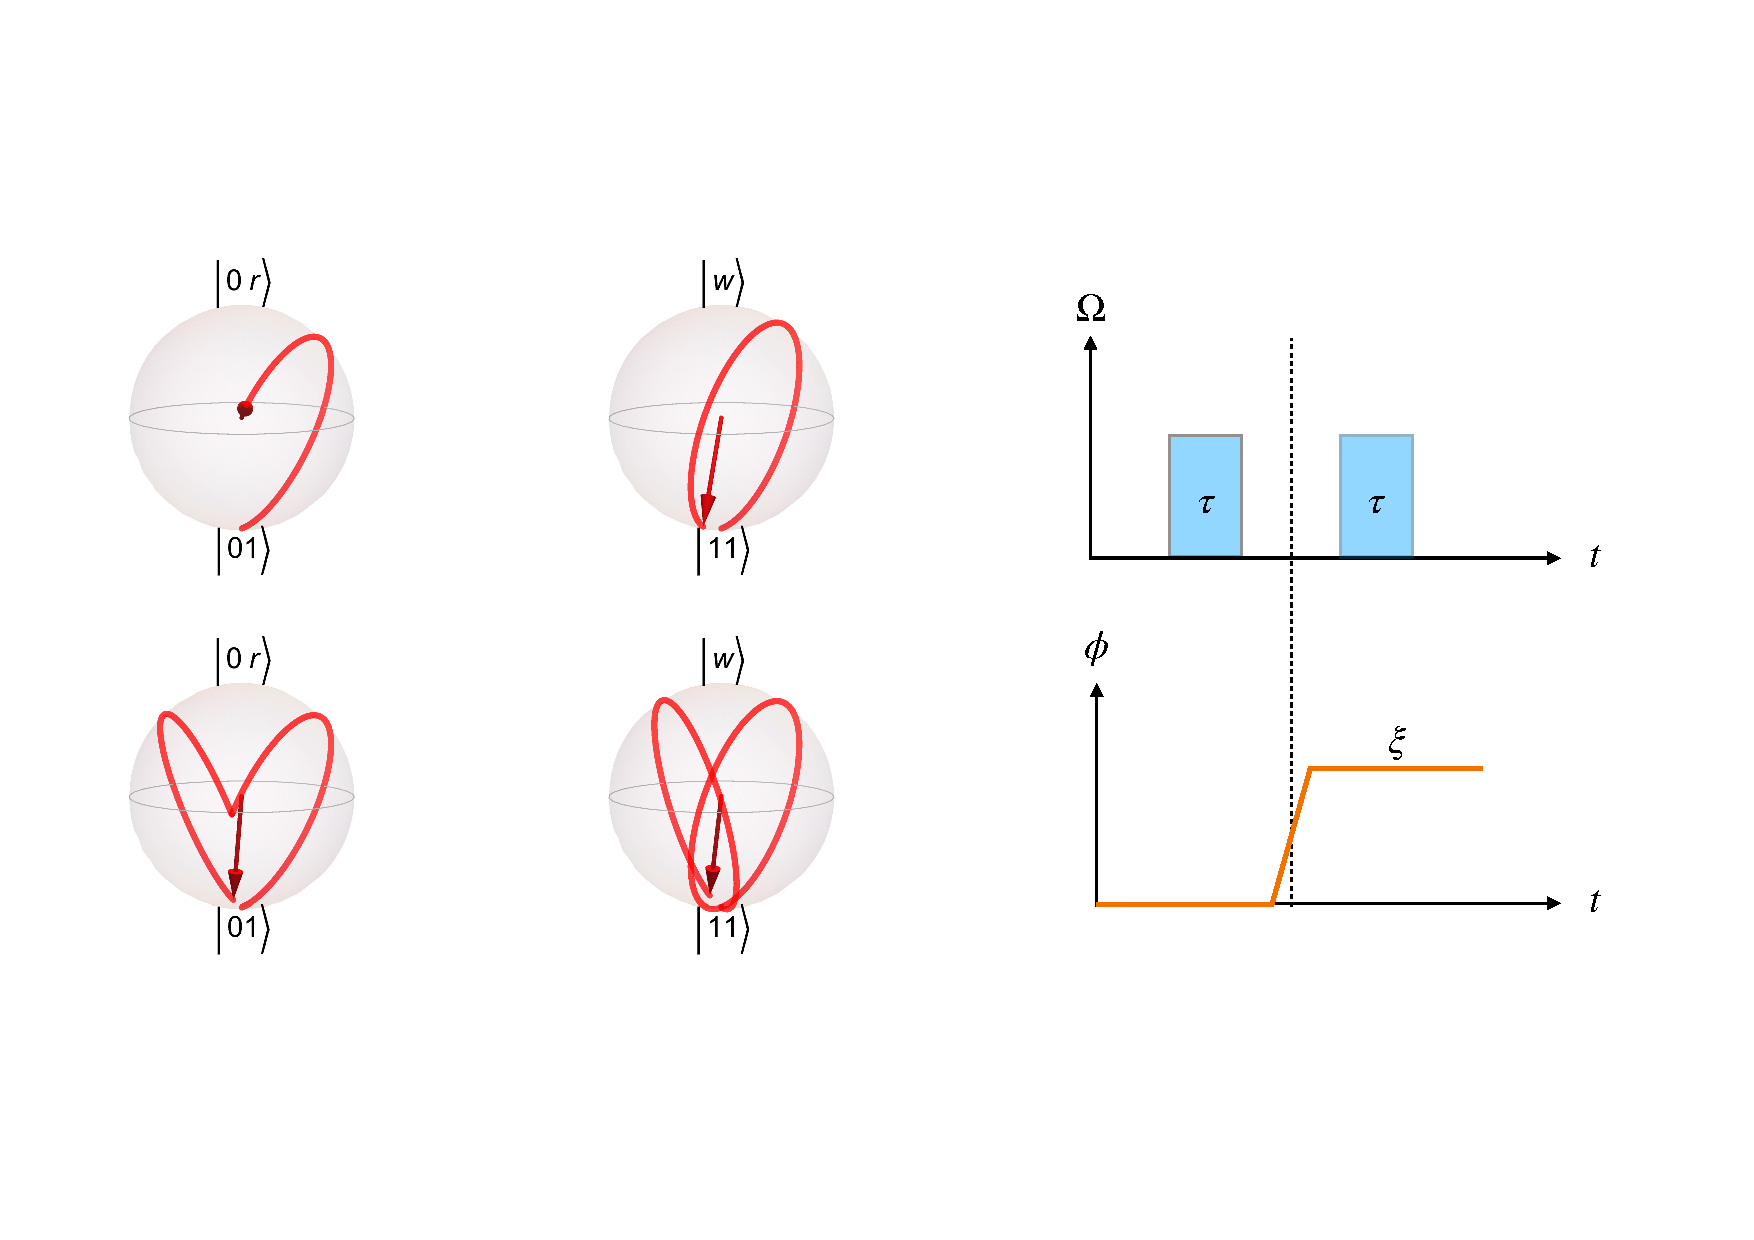
\includegraphics[width=1.0\textwidth]{images/LP_total.pdf}
	\caption{Слева: состояние системы после первого и второго импульсов последовательности Levine-Pichler. Справа: последовательность Levine-Pichler состоит из двух импульсов длительности $\tau$ между которыми фаза лазера меняется на $\xi$.}
	\label{fig:LP_total}
\end{figure}


Следует отметить, что был рассмотрен режим взаимодействия по Ван дер Ваальсу, также ридберговское взаимодействие можно организовать через Фёрстеровские резонансы (Förster resonance), которые получаются при рассмотрении вырожденной теории возмущений. Более подробное обсуждение этих вопросов, а также вычисление сил взаимодействия можно найти в статьях \cite{Saffman_Rydberg1, Saffman_Rydberg2,PhysRevLett.85.2208}. В работах \cite{Chew:2022aa,Urban:2009aa} наблюдается эффект ридберговской блокады, реализованной с помощью Фёрстеровских резонансов. 

Для получения достоверных двухкубитных операций на основе эффекта ридберговской блокады требуется возбуждать атомы в ридберговское состояние с высокой точностью. Далее будут приведены результаты моделирования двухфотонного возбуждения в ридберговское состояние с учётом основных источников ошибок: теплового движения атома в оптическом пинцете, спонтанного распада из промежуточного состояния, фазовых шумов лазера, ошибок приготовления и измерения состояния.

% Будет время - надо вставить картинку величины взаимодействия от расстояния. Построить график с помощью ARC по сути

\subsection{Моделирование двухфотонного ридберговского возбуждения}

Существуют работы \cite{Srakaew:2023aa}, в которых производится однофотонное возбуждение в ридберговское состояние с помощью лазеров с длиной волны в глубоком ультрафиолете ($100-300$ нм), однако использование таких лазеров технически затруднительно. Возникают проблемы с износом оптического оборудования под воздействием УФ-излучения, отсутствием доступных мощных лазеров, быстрым затуханием излучения вне вакуума. Поэтому более популярным подходом является использование двухфотонного возбуждения в каскадной схеме с использованием вспомогательного промежуточного уровня (рис. \ref{fig:CascadeScheme}). Такой подход используется в том числе в нашей установке. 

\begin{figure}[ht]
	\centering
	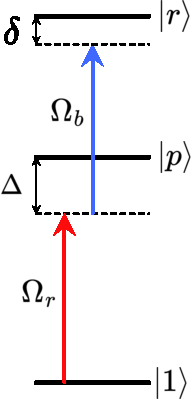
\includegraphics[width=0.2\textwidth]{images/CascadeScheme.pdf}
	\caption{Схема двухфотонного возбуждения в каскадной конфигурации трёхуровневой системы.}
	\label{fig:CascadeScheme}
\end{figure}
	
Теоретическое описание такой трёхуровневой системы с точностью до переобозначений полностью совпадает с расмотренными ранее двухфотонными рамановскими переходами в $\Lambda$-схеме \cite{Steck,Lukin}. Гамильтониан системы в приближении вращающейся волны имеет вид 

\begin{equation}
	\hat{H}=-\Delta\ket{p}\bra{p}-\delta\ket{r}\bra{r}+\frac{\Omega_r}{2}\left(e^{i\phi_r}\ket{1}\bra{p}+e^{-i\phi_r}\ket{p}\bra{1}\right)+\frac{\Omega_b}{2}\left(e^{i\phi_b}\ket{p}\bra{r}+e^{-i\phi_b}\ket{r}\bra{p}\right).
\end{equation}

В нашем эксперименте используются кубитные состояния $\ket{0} = \ket{5^2S_{1/2},F=2,m_F=0}$ и $\ket{1} = \ket{5^2S_{1/2},F=2,m_F=1}$, промежуточный уровень $\ket{p} = \ket{5^2P_{1/2},F=2,m_F=1}$ и ридберговское состояние $\ket{r}=\ket{{72}^2S_{1/2}}$. В схеме ридберговского возбуждения можно выделить следующие источники ошибок:  


\begin{itemize}
	\item динамика атома в оптическом пинцете и эффект Доплера,
	\item спонтанный распад из промежуточного состояния, 
	\item ошибки измерения и приготовления состояния,
	\item фазовые шумы лазера, 
	\item конечное время жизни ридберговского состояния,
	\item возбуждение в соседние ридберговские состояния,
	\item амплитудные шумы лазера,
	\item смещение оптических лучей, 
	\item переотражение лазерных лучей, 
	\item паразитные внешние поля.
\end{itemize}

Ошибки из-за амплитудных шумов лазера и смещения оптических лучей считаются несущественными, так как интенсивность и положение лазеров стабилизируются по дополнительной камере. Перекачка в соседние ридберговские состояния с другой проекцией полного момента $m_J$ \cite{Evered:2023aa} потенциально может происходить, но при сканировании частоты лазеров наблюдается только один двухфотонный резонанс. Конечное время жизни ридберговского состояния можно не учитывать, так как естественное время жизни состояния $\ket{r} = \ket{72^{2}S_{1/2}}$ при комнатной температуре составляет порядка $160\text{ мкс}$ \cite{Ryabtsev_BBR}, что для характерного периода ридберговских осцилляций $1\text{ мкс}$ даёт ошибку на уровне $0.5 \%$. Паразитные электрические поля, вызывающие отстройку атома от резонанса за счёт штарковсих сдивгов (DC Stark shifts), компенсируются с помощью восьми электродов в октупольной конфигурации \cite{Beguin}, расположенных вблизи атомного массива. Такая конфигурация полей позволяет компенсировать напряжения независимо по трём осям, сами поля измеряются по сдвигу ридберговского резонанса, который крайне чувствителен к электрическим полям \cite{Beguin}. При переотражении лазерных пучков в вакуумной камере может создаваться стоячая волна в районе атомного массива, что также служит потенциальным источником ошибок. Так как размер атома в ридберговском состоянии составляет порядка мкм, что по порядку совпадает с длиной волны лазерного излучения в оптическом диапазоне, то изменение электрического поля на масштабе атома за счёт образования стоячей волны потенциально может приводить к ошибкам. Этот механизм  планируется изучить в дальнейшей работе, далее будут рассмотрены  ошибки связанные с тепловым движением атома, фазовыми шумами лазера, спонтанным распадом из промежуточного состояния, а также приготовлением и измерением состояния. 


\subsubsection{Тепловое движение атома в оптическом пинцете}

Моделирование ошибок двухфотонного возбуждения в ридберговское состояние отличается от ранее проделанного моделирования для рамановских однокубитных операций тем, что используется встречная конфигурация лазерных пучков, а также происходит выключение оптической ловушки на время проведения операции. Оптический пинцет выключается, так как в ридберговском состоянии потенциал ловушки становится отталкивающим (anti-trapping) за счёт изменения знака отстройки \cite{Browayes,Beguin,grimm1999optical}. Этот эффект используется для детектирования возбуждения в ридберговское состояние по выбиванию атома из ловушки\cite{Beguin}.


\subsubsection{Спонтанный распад из промежуточного состояния}

\subsubsection{Фазовые шумы лазера}

\subsubsection{Ошибки приготовления и измерения состояния}

\subsection{Измерение параметров модели}

\subsubsection{Гетеродинное измерение спектра фазовых шумов лазеров}


% \begin{figure}
% 	\centering
% 	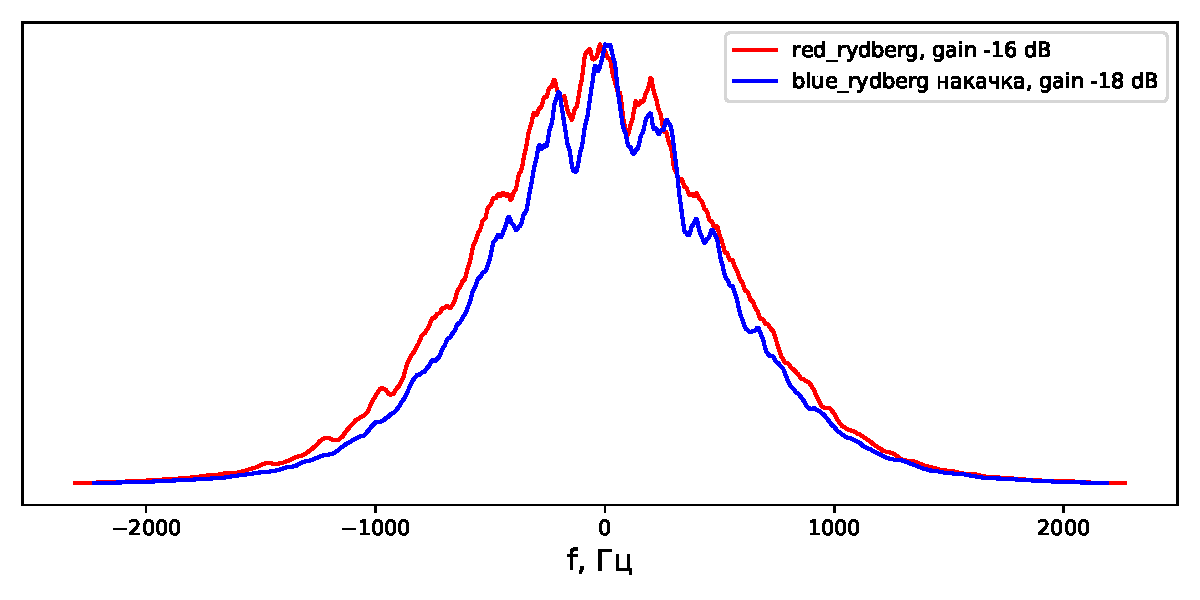
\includegraphics[width=0.75\textwidth]{images/turbo_spectrum.pdf}
% 	\caption{Спектры лазеров, используемых для двухфотонного ридберговского возбуждения при включенном турбонасосе.}
% 	\label{fig:turbo_spectrum}
% \end{figure}

\subsubsection{Измерение SPAM-ошибки}

\subsection{Улучшение двухкубитных вентилей за счёт flat-top пучков}

\subsection{Результаты главы}


\newpage